\documentclass[onecolumn, draftclsnofoot,10pt, compsoc]{IEEEtran}
\usepackage{graphicx}
\usepackage{url}
\usepackage{setspace}

%Personal imports
%\usepackage{cite}

\usepackage{geometry}
\geometry{textheight=9.5in, textwidth=7in}

% 1. Fill in these details
\def \CapstoneTeamName{		Group}
\def \CapstoneTeamNumber{		35}
\def \GroupMemberOne{			Christopher Carlsen}
\def \GroupMemberTwo{			Yizheng Wang}
\def \GroupMemberThree{			Peter Dorich}
\def \CapstoneProjectName{		Develop an Internet of Things Irrigation Valve}
\def \CapstoneSponsorCompany{	 	OSU \textbar\hspace{.05in} Openly Published Environmental Sensing (OPEnS) Lab}
\def \CapstoneSponsorPerson{		Chet Udell}

% 2. Uncomment the appropriate line below so that the document type works
\def \DocType{		%Problem Statement
	Requirements Document
	%Technology Review
	%Design Document
	%Progress Report
}

\newcommand{\NameSigPair}[1]{\par
	\makebox[2.75in][r]{#1} \hfil 	\makebox[3.25in]{\makebox[2.25in]{\hrulefill} \hfill		\makebox[.75in]{\hrulefill}}
	\par\vspace{-12pt} \textit{\tiny\noindent
		\makebox[2.75in]{} \hfil		\makebox[3.25in]{\makebox[2.25in][r]{Signature} \hfill	\makebox[.75in][r]{Date}}}}
% 3. If the document is not to be signed, uncomment the RENEWcommand below
%\renewcommand{\NameSigPair}[1]{#1}

%%%%%%%%%%%%%%%%%%%%%%%%%%%%%%%%%%%%%%%
\begin{document}
	\begin{titlepage}
		\pagenumbering{gobble}
		\begin{singlespace}
			
\includegraphics[height=4cm]{coe_v_spot1}
			\hfill 
			% 4. If you have a logo, use this include graphics command to put it on the coversheet.
			%\includegraphics[height=4cm]{CompanyLogo}   
			\par\vspace{.2in}
			\centering
			\scshape{
				\huge CS461 Capstone \DocType \par
				{\large\today - Fall Term}\par
				\vspace{.5in}
				\textbf{\Huge\CapstoneProjectName}\par
				\vfill
				{\large Prepared for}\par
				\Huge \CapstoneSponsorCompany\par
				\vspace{10pt}
				{\Large\NameSigPair{\CapstoneSponsorPerson}\par}
				{\large Prepared by }\par
				Group\CapstoneTeamNumber\par
				% 5. comment out the line below this one if you do not wish to name your team
				%\CapstoneTeamName\par 
				\vspace{5pt}
				{\Large
					\NameSigPair{\GroupMemberOne}\par
					\NameSigPair{\GroupMemberTwo}\par
					\NameSigPair{\GroupMemberThree}\par
				}
				\vspace{20pt}
			}
			\begin{abstract}
				% 6. Fill in your abstract   --- TODO 
				This document is the Requirements Specification that will be used to detail the objectives of the Internet of Things Irrigation Valve project.
				It will contain a more specific look at what completion goals for this project are and what a user of the this project's product should reasonably expect.
			\end{abstract}     
		\end{singlespace}
	\end{titlepage}
	\newpage
	\pagenumbering{arabic}
	\tableofcontents
	% 7. uncomment this (if applicable). Consider adding a page break.
	%\listoffigures
	%\listoftables
	\clearpage
	
	% 8. now you write!
	\section{Introduction}
	\subsection{Purpose}
	This requirements specification (RS) document serves to more concretely establish the desired end goals of the Irrigation Valve project.
	Its intended usage is for the Irrigation Valve team and their client, Chet Udell, as well as any third party groups with whom may become involved over the course of the project. 
	\subsection{Scope}
	There will be three overall products of this project, defined a follows -\vspace{-.1in}
	\subsubsection{Soil Moisture Sensor/Valve Control}
	The soil moisture sensor's primary job will be to read moisture data from a pre-existing piece of hardware.
	Upon reading this data, it will send it to a designated data-collection hub.
	This device will also embody the "physical" aspect of this project, as it will be the device that engages or disengages an attached valve.
	\subsubsection{Centralized Data Hub/Command Relay}
	This device will be used as the communication go-between device that collects data from the various sensors, and then relays it to a remote data-collection point.
	Its other primary function will be to send instructions passed to it from the user (via the user interface) to individual sensor devices, detailing when a device should be turned on or off.
	\subsubsection{Web-based User Interface/Data Tracker}
	Serving as the "face" of the project, this will be the actual interface with which this system's users will interact.
	The user will use this system to view recorded moisture data from various sensors, as well as use it to make decisions on when and where water is most needed in their field.
	This system will take user input and send it to desired watering schedules (via the relay hub) to the individual sensor/valve-control devices in the desired watering areas.
	\subsection{Definitions, acronyms and abbreviations}
	For purposes of brevity, some abbreviations may be used through out this document as follows:
	\begin{itemize}
		\item{[Sensor/soil sensor/moisture sensor] - Will be used in reference to the "Soil Moisture Sensor/Valve Control" device and its related parts.}
		\item{[Data hub/hub/relay] - Will be used in reference to the "Information Communication Relay/Command" device and its related parts.}
		\item{[UI/Interface/database/tracker] - Will be used in reference to the "Web-based User Interface/Data Tracker" device and its related parts.}
	\end{itemize}
	\subsection{References}
	See Appendix A
	\subsection{Overview}
	
	\section{Overall description}
	\subsection{Product perspective}
	This projects final product, a soil-moisture data tracking and informed irrigation valve control system, will stand as an individual product composed of three parts.
	The product, however, will be included under a blanket project group known as Project Loom.
	It will not be reliant on other Project Loom products for any functionality, but may potentially be considered as a competent part of an overall package delivered by Project Loom.
	
	%TODO - FILL OUT remainder of this section with information regarding
	% a) System interfaces;
	% b) User interfaces;
	% c) Hardware interfaces;
	% d) Software interfaces;
	% e) Communications interfaces;
	% f) Memory;
	% g) Operations;
	% h) Site adaptation requirements;
	% (See section 5.2.1 for more information)
	
	\subsection{Product functions}
	\subsection{User characteristics}
	\subsection{Constraints}
	The following are the design constraints for the Hub portion of the project.
	These constraints are all hardware and software that our client would like to use.
	This preference is because the previous technologies and hardware are already being used in the organization, and are needed in order to maintain compatibility and uniformity.
	\begin{itemize}
		\item{32u4 RFM95 LORA Radio with 915 MHz processors (Sensors and Hub)}
		\item{Ethernet Shield (Hub)}
		\item{Arduino IDE (Sensors and Hub)}
		\item{MQTT (Hub and User Interface)}
	\end{itemize}
	\subsection{Assumptions and dependencies}
	\section{Specific requirements}
	\subsection{Soil Moisture Sensor/Valve Control}
	\begin{itemize}
		\item{As a user, I want the sensor device to that take moisture data samples every 15 minutes.}
		\item{As a user, I want the irrigation valve turned on or off, based on a set of conditionals triggers that I set.}
		\item{As a user, I want a fail-safe/contingency set of instructions that the device will fall back on should it lose contact with the hub device or internet.}
	\end{itemize}
	
	\subsection{Information Communication Relay/Command}
	\begin{itemize}
		\item{As a user, I want the communications between the hub and sensor devices to use a wireless medium.}
		\item{As a user, I want the hub to relay information between the valve and the web application.}
		\item{As a user, I want the hub to send irrigation control information \textit{only} to valve-control devices that I specify.}
		\item{As a user, I want the hub to tell sensor devices which valve-control state that they should use, between:}
		\begin{itemize}
			\item{Valve opens and closes based only on soil moisture data.}
			\item{Valve opens and closes based only on the time of day.}
			\item{Valve opens and closes based on both time of day and moisture data.} 
			\item{(\textbf{Stretch Goal}) Manual only}
		\end{itemize}
	\end{itemize}
	
	\subsection{Web-based User Interface/Data Tracker}
	\begin{itemize}
		\item{As a user, I want to view the collected moisture data from various moisture sensor devices in my field, as well as the position status of connected valves (e.g. open/closed).}
		\item{As a user, I want to use the application interface to set valve activation conditions for specific valve devices.}
	\end{itemize}    
	\section{Gantt chart}
	(This is just a place holder at the moment.)\par
	\noindent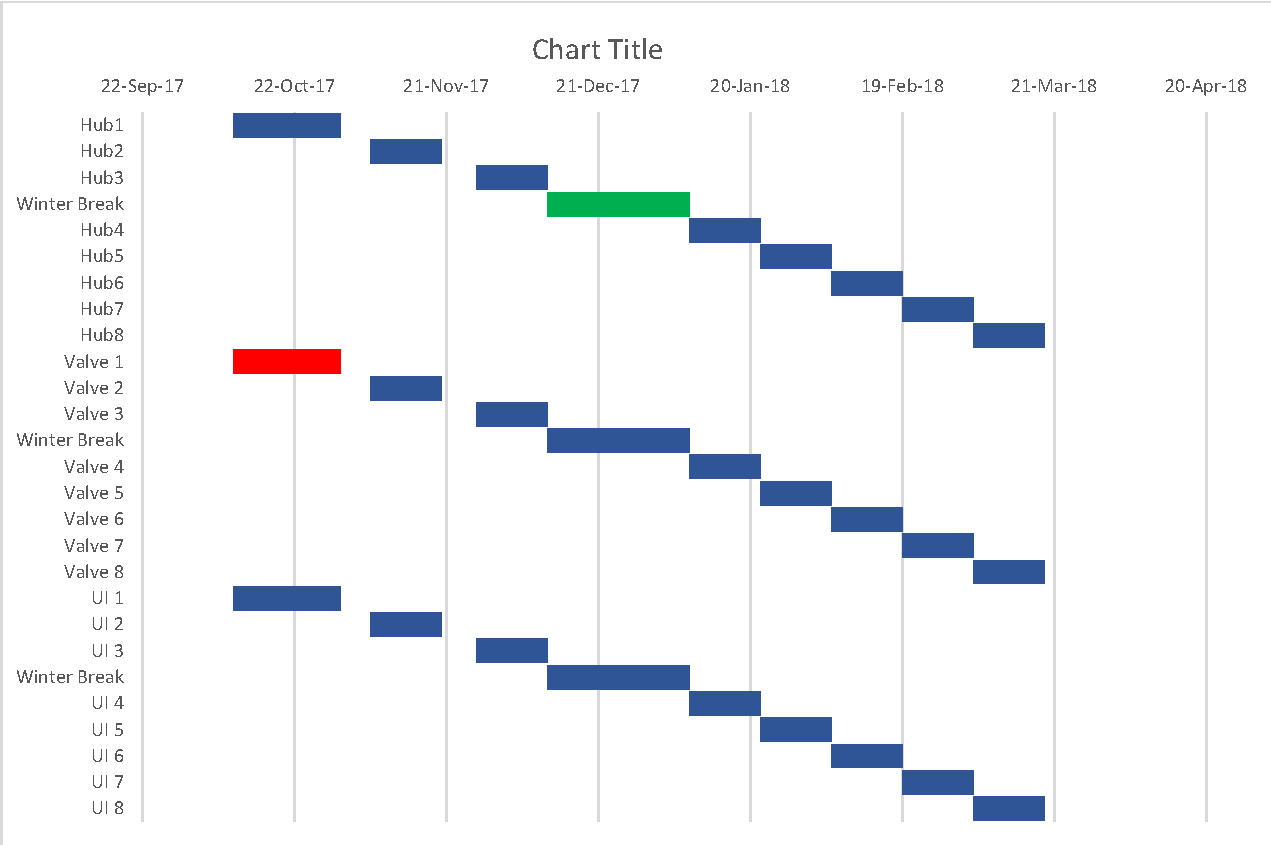
\includegraphics[width=\linewidth]{chart_cropped}
	
	\newpage
	\section{Appendix A - Bibliography}
	\nocite{*} %TODO - Remove this if citing things.
	\bibliographystyle{IEEEtran}
	\bibliography{references}
	
\end{document}